\documentclass[12pt]{article}
\usepackage[utf8]{inputenc}
\usepackage[spanish,es-lcroman, es-tabla]{babel}
\usepackage[autostyle,spanish=mexican]{csquotes}
\usepackage{amsmath}
\usepackage{amssymb}
\usepackage{nccmath}
\numberwithin{equation}{section}
\usepackage{amsthm}
\usepackage{graphicx}
\usepackage{epstopdf}
\DeclareGraphicsExtensions{.pdf,.png,.jpg,.eps}
\usepackage{color}
\usepackage{float}
\usepackage{multicol}
\usepackage{enumerate}
\usepackage[shortlabels]{enumitem}
\usepackage{anyfontsize}
\usepackage{anysize}
\usepackage{array}
\usepackage{multirow}
\usepackage{enumitem}
\usepackage{cancel}
\usepackage{tikz}
\usepackage{circuitikz}
\usepackage{tikz-3dplot}
\usetikzlibrary{babel}
\usetikzlibrary{shapes}
\usepackage{bm}
\usepackage{mathtools}
\usepackage{esvect}
\usepackage{hyperref}
\usepackage{relsize}
\usepackage{siunitx}
\usepackage{physics}
%\usepackage{biblatex}
\usepackage{standalone}
\usepackage{mathrsfs}
\usepackage{bigints}
\usepackage{bookmark}
\spanishdecimal{.}

\setlist[enumerate]{itemsep=0mm}

\renewcommand{\baselinestretch}{1.5}

\let\oldbibliography\thebibliography

\renewcommand{\thebibliography}[1]{\oldbibliography{#1}

\setlength{\itemsep}{0pt}}
%\marginsize{1.5cm}{1.5cm}{2cm}{2cm}


\newtheorem{defi}{{\it Definición}}[section]
\newtheorem{teo}{{\it Teorema}}[section]
\newtheorem{ejemplo}{{\it Ejemplo}}[section]
\newtheorem{propiedad}{{\it Propiedad}}[section]
\newtheorem{lema}{{\it Lema}}[section]

\usepackage{mathrsfs}
\usepackage{bigints}
%\usepackage{enumerate}
%\author{M. en C. Gustavo Contreras Mayén. \texttt{curso.fisica.comp@gmail.com}}
\title{Función Gamma y Función Beta \\ {\large Matemáticas Avanzadas de la Física}}
\date{ }
\begin{document}
%\renewcommand\theenumii{\arabic{theenumii.enumii}}
\renewcommand\labelenumii{\theenumi.{\arabic{enumii}}}
\maketitle
\fontsize{14}{14}\selectfont
%Referencia Arfken Capítulo 8. Función Gamma.
La función gamma aparece ocasionalmente en problemas físicos tales como la normalización de las funciones de onda de Coulomb y el cálculo de probabilidades en mecánica estadística.
\par
En general, sin embargo, tiene una aplicación e interpretación física menos directa que, por ejemplo, las funciones de Legendre y Bessel. Más bien, su importancia radica en su utilidad para desarrollar otras funciones que tienen una aplicación física directa.
\section{Función Gamma}
Existen al menos tres formas convenientes de definir la función Gamma.
\subsection{Límite infinito (Euler)}
La primera definición, llamada de \emph{Euler} es
\begin{equation}
\Gamma(z) \equiv \lim_{n \to \infty} \dfrac{1 \cdot 2 \cdot 3 \cdots n}{z (z+1) (z+2) \cdots (z+n)} n^{z}, \hspace{1.5cm} z \neq	0, -1,-2,-3, \ldots
\label{eq:ecuacion_10_01}
\end{equation}
Esta definición de $\Gamma(z)$ es útil para el desarrollo del producto infinito de Weierstrass de $\Gamma (z)$. Sin pérdida de generalidad, $z$ puede ser real o complejo. Re-emplazando $z$ con $z + 1$, tenemos
\begin{align}
\begin{aligned}
\Gamma (z + 1) &= \lim_{n \to \infty} \dfrac{1 \cdot 2 \cdot 3 \cdots n}{(z + 1)(z + 2)(z + 3) \cdots (z + n + 1)} n^{z + 1} \\
&= \lim_{n \to \infty} \dfrac{n \, z}{z + n + 1} \: \dfrac{1 \cdot 2 \cdot 3 \cdots n}{z (z + 1)(z + 2)(z + 3) \cdots (z + n)} n^{z} \\
&= z \: \Gamma (z)
\label{eq:ecuacion_10_02}
\end{aligned}
\end{align}
Esta es la relación funcional básica para la función gamma. Debe notarse que es una ecuación de diferencias. Se ha demostrado que la función gamma es una de una clase general de funciones que no satisfacen ninguna ecuación diferencial con coeficientes racionales.
\par
Específicamente, la función gamma es una de las pocas funciones de la física matemática que no satisface ni la ecuación diferencial hipergeométrica ni la ecuación hipergeométrica confluente.
\par
De la definición
\begin{align}
\Gamma (1) = \lim_{n \to \infty} \dfrac{1 \cdot 2 \cdot 3 \cdots n}{1 \cdot 2 \cdot 3 \cdots n \, (n + 1)} \: n = 1
\label{eq:ecuacion_10_03}
\end{align}
Usando de la ecuación (\ref{eq:ecuacion_10_02}), tenemos
\begin{align}
\begin{aligned}
\Gamma (2) &= 1 \\
\Gamma (3) &=  2 \: \Gamma(2) =  2 \\
\Gamma (n) &= 1 \cdot 2 \cdot 3 \cdots (n-1) =  (n-1)!
\label{eq:ecuacion_10_04}
\end{aligned}
\end{align}
\subsection{Integral definida (Euler)}
Una segunda definición es la llamada integral de Euler:
\begin{equation}
\Gamma (z) \equiv \int_{0}^{\infty} e^{-t} \: t^{z - 1} \, \dd t, \hspace{1.5cm} \Re(z) > 0
\label{eq:ecuacion_10_05}
\end{equation}
La restricción en $z$ es necesaria para prevenir la divergencia de la integral. Cuando la función Gamma aparece en problemas de la física, a menudo tiene una variante
\begin{align}
\Gamma (z) &= 2 \: \int_{0}^{\infty} \exp(-t^{2}) \: t^{2 \, z - 1} \dd t, \hspace{1.5cm} \Re(z) > 0  \label{eq:ecuacion_10_06} \\
\Gamma (z) &=  \int_{0}^{1} \left[ \ln\left(\dfrac{1}{t} \right) \right]^{z - 1} \dd t, \hspace{1.5cm} \Re (z) > 0 \label{eq:ecuacion_10_07}
\end{align}
Cuando $z=1/2$, la ecuación (\ref{eq:ecuacion_10_06}) es la función de error gaussiana, que nos devuelve el siguiente resultado interesante:
\begin{equation}
\Gamma (1/2) = \sqrt{\pi}
\label{eq:ecuacion_10_08}
\end{equation}
Para mostrar la equivalencia de esas dos definiciones, las ecuaciones (\ref{eq:ecuacion_10_01}) y (\ref{eq:ecuacion_10_05}) consideremos la función de dos variables
\begin{equation}
F(z, n) = \int_{0}^{n} \left( 1 - \dfrac{t}{n} \right)^{n} \: t^{z - 1} \dd t, \hspace{1.5cm} \Re(z) > 0
\label{eq:ecuacion_10_09}
\end{equation}
con $n$ entero positivo. Ya que
\begin{equation}
\lim_{n \to \infty} \left( 1 - \dfrac{t}{n} \right)^{n} \equiv e^{-t}
\label{eq:ecuacion_10_10}
\end{equation}
de la definición de función exponencial
\begin{equation}
\lim_{n \to \infty} F(z, n) = F(z, \infty) = \int_{0}^{\infty} \exp(-t) \: t^{z - 1} \dd t \equiv \Gamma (z)
\label{eq:ecuacione_10_11}
\end{equation}
por la ecuación (\ref{eq:ecuacion_10_05}).
\\
Regresando a $F(z,n)$, evaluamos sucesivamente la integral por partes, hacemos de manera conveniente $u = t/n$. Entonces
\begin{equation}
F(z,n) = n^{2} \: \int_{0}^{1} (1-u)^{n} \: u^{z-1} \dd u
\label{eq:ecuacione_10_12}
\end{equation}
Integrando por partes
\begin{equation}
\dfrac{F(z, n)}{n^{2}} =  (1-u)^{n} \: \dfrac{u^{z}}{z} \Bigg\vert_{0}^{1} + \dfrac{n}{z} \: \int_{0}^{1} (1-u)^{n-1} \: u^{z} \dd u
\label{eq:ecuacion_10_13}
\end{equation}
Repitiendo esto cada vez con el integrando se anula en ambos extremos, por lo que
\begin{align}
\begin{aligned}
F(z,n) &= n^{z} \: \dfrac{n(n-1) \cdots 1}{z \, (z+1) \cdots (z+n-1)} \int_{0}^{1} u^{z+n-1} \, \dd u \\
&= \dfrac{1 \cdot 2 \cdot 3 \cdots n}{z \, (z+1)(z+2) \cdots (z+n)} \: n^{z}
\label{eq:ecuacion_10_14}
\end{aligned}
\end{align}
Que es idéntico con la expresión del lado derecho de la ecuación (\ref{eq:ecuacion_10_01}). De aquí que
\begin{equation}
\lim_{n \to \infty} F(z, n) = F(z, \infty) \equiv \Gamma (z)
\label{eq:ecuacion_10_15}
\end{equation}
\subsection{Producto infinito (Weierstrass)}
La tercera forma conocida como forma de Weierstrass es
\begin{equation}
\dfrac{1}{\Gamma (z)} \equiv z \:  e^{\gamma \, z} \: \prod_{n=1}^{\infty} \left( 1 + \dfrac{z}{n} \right) \: e^{-z/n}
\label{eq:ecuacion_10_16}
\end{equation}
donde $\gamma$ es la constante de \emph{Euler-Mascheroni}
\begin{equation}
\gamma = 0.5772156619
\label{eq:ecuacion_10_17}
\end{equation}
De esta definición de producto infinito de $\Gamma (z)$, se obtiene una identidad importante:
\begin{equation}
\Gamma (z) \: \Gamma (1 - z) = \dfrac{\pi}{\sin z \, \pi}
\label{eq:ecuacion_10_23}
\end{equation}
Así también la \textbf{fórmula de duplicación de Legendre}:
\begin{equation}
\Gamma (1 + z) \: \Gamma (z + \frac{1}{2}) = 2^{-2 \, z} \: \sqrt{\pi} \: \Gamma (2 \, z + 1)
\label{eq:ecuacion_10_24b}
\end{equation}
La definición de Weierstrass muestra directamente que $\Gamma (z)$ tiene polos sencillos en $z = 0, -1, -2, -3, \ldots$ y que $[\Gamma (z)]^{-1}$ no tiene polos en el plano complejo, lo que significa que $\Gamma (z)$ no tiene ceros.
\subsection{Notación factorial}
El valor de $-1$ en el exponente $z-1$ de la segunda definición (ecuación \ref{eq:ecuacion_10_05}) es una molestia continua, podemos re-escribir
\begin{equation}
\int_{0}^{\infty} e^{-t} \: t^{z} \: \dd t \equiv z!,  \hspace{1.5cm} \Re (z) > 0
\label{eq:ecuacion_10_25}
\end{equation}
que define la \emph{función factorial} $z!$. A veces se puede encontrar escrita con la notación de Gauss: $\prod (z)$ como
\begin{equation}
\prod(z) = z! = \Gamma (z + 1)
\label{eq:ecuacion_10_26}
\end{equation}
donde la notación $\Gamma$ se debe a Legendre. La función factorial de la ecuación (\ref{eq:ecuacion_10_25}) está relacionada con la función Gamma
\begin{equation}
\Gamma (z) = (z-1)! \hspace{1cm} \mbox{ o } \hspace{1cm} \Gamma (z + 1) = z!
\label{eq:ecuacion_10_27}
\end{equation}
Si $z=n$, un entero positivo (ecuación \ref{eq:ecuacion_10_04}), se demuestra que
\begin{equation}
z! = n! = 1 \cdot 2 \cdot 3 \cdots n
\label{eq:ecuacion_10_28}
\end{equation}
que el la forma conocida del factorial. Sin embargo, hay que tomar en cuenta que como $z!$ ahora está definido por la eq. (\ref{eq:ecuacion_10_25}) (o de forma equivalente por la ecuación (\ref{eq:ecuacion_10_27})) la función factorial ya no está limitada a valores positivos del argumento de las integrales (figura \ref{fig:figura_10_01}).
\begin{figure}[H]
    \centering
    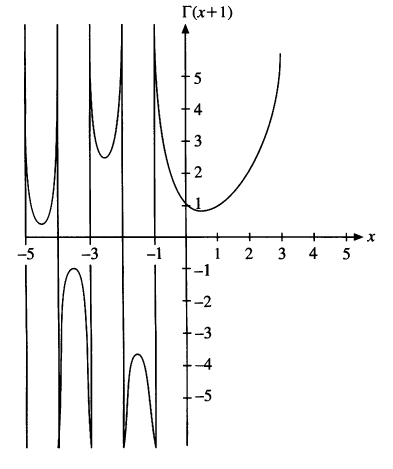
\includegraphics[scale=0.6]{Imagenes/FuncionFactorial_01.png}
    \caption{La función factorial. Extensión a los argumentos negativos.}
    \label{fig:figura_10_01}
\end{figure}
La relación de diferencias (ec. (\ref{eq:ecuacion_10_02})) se convierte
\begin{equation}
(z - 1)! = \dfrac{z!}{z}
\label{eq:ecuacion_10_29}
\end{equation}
Esto muestra de inmediato que
\begin{equation}
0!= 1
\label{eq:ecuacion_10_30}
\end{equation}
y además
\begin{equation}
n! = \pm \infty \hspace{2cm} \mbox{para $n$, un \textbf{entero negativo.}}
\label{eq:ecuacion_10_31}
\end{equation}
\subsection{Notación doble factorial}
En varios problemas de la física, en particular con los polinomios de Legendre, encontraremos productos de enteros impares positivos y de pares positivos, por conveniencia, definimos el doble factorial:
\begin{align}
\begin{aligned}
1 \cdot 3 \cdot 5 \cdots (2 \, n+1) &= (2 \, n+1) !! \\
2 \cdot 4 \cdot 6 \cdots (2 \, n) &= (2 \, n) !!
\end{aligned}
\label{eq:ecuacion_10_33b}
\end{align}
Que están relacionados con la función factorial
\begin{equation}
(2 \, n)!! =  2^{n} \: n! \hspace{1cm} \mbox{ y } \hspace{1cm} (2 \, n+1)!! = \dfrac{(2 \, n+1)!}{2^{n} \, n!}
\label{eq:ecuacion_10_33c}
\end{equation}
También definimos $(-1)!! = 1$, un caso especial que no se obtiene de la ec. (\ref{eq:ecuacion_10_33c})
\subsection{Algunas cosas sobre la función Gamma.}
Es posible calcular el valor de la función Gamma para todos los números naturales y semienteros positivos. Para $z \in \mathbb{N}$ tenemos
\begin{align*}
\begin{aligned}
\Gamma (z+1) &= z \: \Gamma (z) \\
\Gamma (2) &= \Gamma (1+1) = \Gamma (1) \\
\Gamma (3) &= \Gamma (2+1) = 2 \: \Gamma (2)= 2 \cdot 1 = 2! \\
\Gamma (4) &= \Gamma (3+1) = 3 \: \Gamma (3)= 3 \cdot 2 = 3! \\
\vdots \\
\Gamma (n) &= \Gamma (n-1+1) = (n-1) \: \Gamma (n-1)= (n - 1) \cdot (n - 2)! = (n-1)!
\end{aligned}
\end{align*}
Para los números semienteros de la forma $2n+1/2, \mbox{ con } n \in \mathbb{Z}$, es decir: $\ldots, -\frac{3}{2}, - \frac{1}{2}, \frac{1}{2}, \frac{3}{2}, \ldots$, tenemos que
\begin{align*}
\begin{aligned}
\Gamma \left( \dfrac{3}{2} \right) &= \Gamma \left( \dfrac{1}{2} + 1 \right) = \dfrac{1}{2} \: \Gamma \left( \dfrac{1}{2} \right) = \dfrac{\sqrt{\pi}}{2} \\
\Gamma \left( \dfrac{5}{2} \right) &= \Gamma \left( \dfrac{3}{2} + 1 \right) = \dfrac{3}{2} \: \Gamma \left( \dfrac{3}{2} \right) = \dfrac{3 \sqrt{\pi}}{4} \\
\vdots \\
\Gamma \left( \dfrac{2n + 1}{2} \right) &= \Gamma \left( \dfrac{2n - 1}{2} + 1 \right) = \dfrac{2n - 1}{2} \; \dfrac{2n - 3}{2} \ldots \dfrac{1}{2} \: \sqrt{\pi} = \dfrac{\sqrt{\pi}}{2^{n}} \; 1 \cdot 3 \ldots (2n-1) \\
\mbox{con } n \in \mathbb{N}
\end{aligned}
\end{align*}
\section{La función Beta.}
Usando la definición integral ec. (\ref{eq:ecuacion_10_25}), podemos escribir el producto de dos factoriales como el producto de dos integrales, y si tomamos las integrales sobre intervalos finitos, se nos facilita el cambio de variables:
\begin{equation}
m! \: n! = \lim_{a^{2} \to \infty} \int_{0}^{a^{2}} e^{-u} \: u^{m} \: \dd u \: \int_{0}^{a^{2}} e^{-v} \: v^{n} \: \dd v \hspace{1cm} \Re (m) > -1, \Re (n) > -1
\label{eq:ecuacion_10_56a}
\end{equation}
Re-emplazando $u$ por $x^{2}$ y $v$ por $y^{2}$, tenemos
\begin{equation}
m! \: n! =  \lim_{a \to \infty} 4 \: \int_{0}^{a} e^{-x^{2}} \: x ^{2 \, m+1} \: \dd x \: \int_{0}^{a} e^{-y^{2}} \: y^{2 \, n+1} \: \dd y
\label{eq:ecuacion_10_56b}
\end{equation}
Transformando a coordenadas polares
\begin{align}
\begin{aligned}
m! \: n! &= \lim_{a \to \infty} 4 \: \int_{0}^{a} e^{-r^{2}} \: r^{2 \, m + 2 \, n+3} \: \dd r \: \int_{0}^{\pi/2} \cos^{2m+1} \theta \: \sin^{2n+1} \theta \dd \theta \\
&= (m+n+1)! \: 2 \: \int_{0}^{\pi/2} \cos^{2m+1} \theta \: \sin^{2n+1} \: \theta \dd \theta
\label{eq:ecuacion_10_58}
\end{aligned}
\end{align}
donde el elemento de área cartesiano $\dd x \: \dd y$ fue re-emplazado por $r \: \dd r \: \dd \theta$.
\begin{figure}[H]
    \centering
    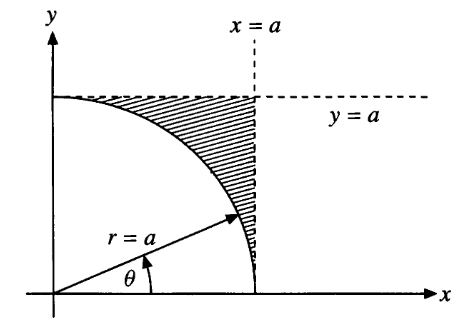
\includegraphics[scale=0.5]{Imagenes/FuncionBeta_01.png}
    \caption{Transformación de coordenadas cartesianas a polares.}
    \label{fig:figura_10_06}
\end{figure}
A la integral definida junto con el factor $2$, se le llama \emph{función Beta}
\begin{align}
\begin{aligned}
B(m+1, n+1) &\equiv 2 \: \int_{0}^{\pi/2} \cos^{2m+1} \theta \: \sin^{2n+1} \: \theta \: \dd \theta \\
&= \dfrac{m! \: n!}{(m+n+1)!} = B(n+1, m+1)
\label{eq:ecuacion_10_58a}
\end{aligned}
\end{align}
Expresada en términos de la función Gamma
\begin{equation}
B(p, q) = \dfrac{\Gamma(p) \: \Gamma(q)}{\Gamma(p+q)}, \hspace{1.5cm} B(q, p) = B(p, q)
\label{eq:ecuacion_10_58b}
\end{equation}
La única razón para elegir $m + 1$ y $n + 1$, en lugar de $m$ y $n$, como argumentos de $B$, es para estar de acuerdo con la convencional función Beta.
\subsection{Formas alternas: integrales definidas.}
La función Beta es útil para la evaluación de una amplia variedad de integrales definidas. Al sustituir $t= \cos^{2} \theta$, la ecuación (\ref{eq:ecuacion_10_58a}) queda como
\begin{equation}
B(m+1, n+1) = \dfrac{m! \: n!}{(m+n+1)!} = \int_{0}^{1} t^{m} \: (1 - t)^{n} \: \dd t
\label{eq:ecuacion_10_59a}
\end{equation}
Re-emplazando $t$ por $x^{2}$, obtenemos
\begin{equation}
\dfrac{m! \: n!}{2 \, (m+n+1)!} = \int_{0}^{1} x^{2m+1} \: (1-x^{2})^{n} \: \dd x
\label{eq:ecuacion_10_59b}
\end{equation}
Al sustituir $t= u/(1+u)$ en la ecuación (\ref{eq:ecuacion_10_59a}), nos proporciona otra expresión útil
\begin{equation}
\dfrac{m! \: n!}{(m+n+1)!} = \int_{0}^{\infty} \dfrac{u^{m}}{(1+u)^{m+n+2}} \: \dd u
\label{eq:ecuacion_10_60}
\end{equation}
%avance revisado.
\subsection{La función Beta incompleta.}
Veremos que como la función Gamma, la función Beta también tiene una definición ''incompleta''
\begin{eqnarray}
\begin{aligned}
B_{x}(p,q) = \int_{0}^{x} t^{p-1} (1-p)^{q-1} dt \hspace{1.5cm} & 0 \leq x \leq 1 \\
& p > 0 \\
& q > 0 (\text{ si } x=1)
\label{eq:ecuacion_10_67}
\end{aligned}
\end{eqnarray}
Cuando $B_{x=1}(p,q)$ se recupera la forma regular (completa) de la función Beta.
\section{Ejemplo con la función Gamma.}
Determine el período de oscilación $\tau$ en función de la energía, para el movimiento de una partícula de masa $m$ en un campo cuya energía potencial es
\[  U = A \vert x \vert^{n}  \]
Para una partícula en este potencial, tenemos que la energía del sistema está dada por
\[ E = \dfrac{1}{2} m \dot{x}^{2} +  A \vert x \vert^{n} \]
Sabemos de la mecánic clásica que para obtener el período del movimiento de una partícula, debemos escribir primero la ecuación anterior en términos de la velocidad
\[ \dot{x}^{2} = \dfrac{2}{m} \left( E - A \vert x \vert^{n} \right) \Rightarrow \dfrac{dx}{dt} =  \sqrt{\dfrac{2}{m}} \sqrt{\left( E - A \vert x \vert^{n} \right)} \]
y después separar la parte de la ecuación dependiente del tiempo, respecto de la parte dependiente de la posición
\[ dt = \dfrac{dx}{\sqrt{\dfrac{2}{m}} \sqrt{\left( E - A \vert x \vert^{n} \right)}} \]
Tomemos en cuenta que todos los potenciales del tipo $U = A \vert x \vert^{n}$ son funciones pares $U(x) =  U(-x)$. Así que para calcular el período de oscilación, que es igual a 2 veces la amplitud, basta con calcular el período de $0$ a $x_{0}$ (donde $\vert x \vert = x$) y se multiplica por cuatro. El punto de retorno $x_{0}$ tiene la propiedad de que la velocidad se anula, esto es
\[ \dot{x_{0}} = 0 \Rightarrow E = A x_{0}^{n} \Rightarrow x_{0} = \left( \dfrac{E}{A} \right)^{1/n} \]
Con lo que
\[ \tau =  4 \sqrt{\dfrac{m}{2}} \bigintss_{0}^{x_{0}} \dfrac{dx}{\sqrt{\dfrac{2}{m}} \sqrt{\left( E - A \vert x \vert^{n} \right)}} = 2 \sqrt{2m} \bigintss_{0}^{(\frac{E}{A})^{1/n}} \dfrac{dx / \sqrt{E}}{\sqrt{(1 - \frac{A}{E} x^{n})}} \]
Haciendo el cambio de variable
\begin{eqnarray}
\begin{aligned}
y &= \left( \dfrac{A}{E} \right)^{1/n} \; x \\
dx &= \left( \dfrac{E}{A} \right)^{1/n} \; dy
\end{aligned}
\end{eqnarray}
por lo que los límites de integración ahora son
\begin{eqnarray}
\begin{aligned}
x = 0 & \Rightarrow y = 0 \\
x = \left( \dfrac{E}{A} \right)^{1/n} & \Rightarrow y = 1
\end{aligned}
\end{eqnarray}
sustituyendo ahora $y^{n} = u$ (ya que $y = u^{1/n} \Rightarrow dy = \frac{1}{n} u^{1/n - 1})$, la integral se reduce a una función Beta
\[ \tau = \dfrac{2}{n} \sqrt{\dfrac{2m}{E}} \left( \dfrac{E}{A} \right)^{1/n} \bigintss_{0}^{1} \dfrac{u^{1/n -1}}{\sqrt{1 - u}} du  = \dfrac{2}{n} \sqrt{\dfrac{2m}{E}} \left( \dfrac{E}{A} \right)^{1/n} B(\dfrac{1}{n}, \dfrac{1}{2}) \]
y como la función Beta se puede expresar con funciones Gamma, resulta
\[ \tau = \dfrac{2}{n} \sqrt{\dfrac{2m}{E}} \left( \dfrac{E}{A} \right)^{1/n} \; \dfrac{\Gamma \left( \frac{1}{n} \right) \Gamma \left( \frac{1}{2} \right) }{\Gamma \left( \frac{1}{2} + \frac{1}{n} \right)} \]
ya sabemos que $\Gamma (1/2) = \sqrt{\pi}$, finalmente llegamos a
\[ \tau = \dfrac{2}{n} \sqrt{\dfrac{2 \pi m}{E}} \left( \dfrac{E}{A} \right)^{1/n} \; \dfrac{\Gamma \left( \frac{1}{n} \right) \Gamma \left( \frac{1}{2} \right) }{\Gamma \left( \frac{1}{2} + \frac{1}{n} \right)} \]
Si $n = 1 \mbox{ con } A > 0$, resulta
\[ \tau = 2 \sqrt{\dfrac{2 \pi m }{E}} \left( \dfrac{E}{A} \right) \dfrac{\Gamma (1)}{\Gamma (\frac{3}{2})} =  \dfrac{4}{A} \sqrt{2mE} \]
para $n = 2$
\[ \tau = \dfrac{2}{2} \sqrt{\dfrac{2 \pi m }{E}} \left( \dfrac{E}{A} \right)^{1/2} \dfrac{\Gamma (\frac{1}{2})}{\Gamma (1)}  =  \pi \sqrt{\dfrac{2m}{A}} \]
Para un oscilador armónico, el período no depende de $E$.
\subsection{Función Gamma para números negativos.}
Si queremos calcular el valor de la función Gamma para un número real negativo $x$ en el intervalo $x \in (-1, 0)$, usamos la relación
\[ \Gamma (z) = \dfrac{\Gamma (z+1)}{z} \]
si  $x = - \frac{1}{2}$, se tiene
\[ \Gamma \left( - \dfrac{1}{2} \right) = \dfrac{\Gamma \left( - \frac{1}{2} + 1 \right) }{- \frac{1}{2}} =  - 2 \Gamma \left( \dfrac{1}{2} \right) = - 2  \sqrt{\pi} \]
Si ahora queremos calcular el valor de la función Gamma, para un número real negativo $x$ en $x \in (-2, -1)$, usamos la relación:
\[ \Gamma (z + 1) = \dfrac{\Gamma (z + 2)}{z + 1} \Rightarrow \Gamma (z) = \dfrac{\Gamma (z + 2)}{z (z + 1)} \]
donde $\Gamma (z + 2) $ es válida para $Re(z) > -2$. Aquí aparecen explícitamente dos polos en la función, uno en $z=0$ y el otro en $z=-1$.
Si $x = - \frac{3}{2}$, resulta
\[ \Gamma \left( - \dfrac{3}{2} \right) = \dfrac{\Gamma \left( - \frac{3}{2} + 2 \right) }{- \frac{3}{2} (- \frac{3}{2} +  1)} =  \dfrac{4}{3} \Gamma \left( \dfrac{1}{2} \right) = \dfrac{4}{3} \sqrt{\pi } \]
y así sucesivamente.

\end{document}